% -------------------------------------------------------------------- %
% -------------------------------------------------------------------- %
% -------------------------------------------------------------------- %
\documentclass{article}
\usepackage[a4paper,
            bindingoffset=0.2in,
            left=1in,
            right=1in,
            top=1in,
            bottom=1in,
            footskip=.25in]{geometry}
\usepackage[utf8]{inputenc}
\usepackage[T1]{fontenc}
\usepackage{csquotes}
\usepackage[english]{babel}
\usepackage{textcomp}
\usepackage{siunitx}
\usepackage[normalem]{ulem}
\usepackage{amsmath}
\usepackage{amssymb}
\usepackage{mhchem}
\usepackage{subcaption}
\usepackage{booktabs}
% Bibliography stuff
\usepackage{biblatex}
\addbibresource{references.bib}
% Diagram stuff
\usepackage{tikz}
\usetikzlibrary{shapes.geometric, arrows}

\renewenvironment{abstract}%
              {% - begin definition
               \small% - select font
               {\bfseries \abstractname}% - select font
               \par% - end a paragraph (skip \parsep)
               \vspace{10pt}% - add vertical space
              }% - complete definition

\renewcommand\abstractname{Abstract}

\pagenumbering{arabic}

% For compatibility between papers and thesis these are redefined in thesis
\newcommand{\sectionOne}[1]{\section{#1} \addvspace{10pt}}
\newcommand{\sectionTwo}[1]{\subsection{#1} \addvspace{10pt}}
\newcommand{\sectionThree}[1]{\subsubsection{#1} \addvspace{10pt}}

%Reviewer Colors
\usepackage{xcolor}
\definecolor{revOne}{HTML}{cc0000}
\definecolor{revTwo}{HTML}{cc9900}
\definecolor{revThree}{HTML}{238E23}
\definecolor{editor}{HTML}{0057fa}
\definecolor{generalColor}{HTML}{ff5733}

%\newcommand{\revised}[2]{\textcolor{#2}{#1}}  % add
%\newcommand{\former}[2]{\textcolor{#2}{\sout{#1}}}
\newcommand{\revised}[2]{#1}  % add

% Commonly used definitions
\def\cantera{\texttt{Cantera}}
\def\nreactions{\Phi}
\def\gasreactions{\tau}
\def\surfreactions{\theta}
\def\nspecies{\Psi}
\def\gasspecies{\lambda}
\def\surfspecies{\mu}
\def \bmh{5pt} %bmatrix height
\def \bmw{5pt} %bmatrix width
\newcommand{\pderv}[2]
{
    \frac{\partial #1}{\partial #2}
}
\newcommand{\jacsurfline}[1]
{
    \pderv{#1}{T} & \pderv{#1}{n_1} &
    \cdots & \pderv{#1}{n_\gasspecies}  & \pderv{#1}{s_{\gasspecies + 1}} &
    \cdots & \pderv{#1}{s_\surfspecies}\\[\bmh]
}
\newcommand{\dotsline}
{
    \vdots & \vdots &
    \ddots & \vdots & \vdots &
    \ddots & \vdots \\[\bmh]
}
\def\cantera{\texttt{Cantera}}
\def\sundials{\texttt{Sundials}}
\def\cvodes{\texttt{CVODES}}
\def\gmres{\texttt{GMRES}}
\def\spgmr{\texttt{SPGMR}}
\def\psolve{\texttt{PSolve}}
\def\eigen{\texttt{Eigen}}
\def\S{\mathcal{S}}
\def\C{\mathcal{C}}
\def\AP{\mathcal{P}}
\def\prodSpecies{\beta}
\def\reactSpecies{\alpha}
\newcommand{\F}[1]{\mathcal{F}(#1)}
\newcommand{\N}[2][]{\mathcal{N}^{#1}(#2)}
\newcommand{\J}[2][]{\mathcal{J}^{#1}(#2)}
\newcommand{\K}[2][]{\mathcal{K}^{#1}(#2)}
\newcommand{\R}[2][]{\mathcal{R}^{#1}(#2)}
\newcommand{\MP}[2][]{\mathcal{P}^{#1}(#2)}
\newcommand{\B}[2][]{\mathcal{B}^{#1}(#2)}
\DeclareSIUnit\concentration{\kilo\mole\per\meter\cubed}
\DeclareSIUnit\ratelaw{\kilo\mole\per\meter\cubed\per\second}
\DeclareSIUnit\mass{\kilo\gram}
\DeclareSIUnit\temperature{\kelvin}
\DeclareSIUnit\atm{atm}
\DeclareSIUnit\bar{bar}
\def\srate{\si{\kilo\mole\per\meter\squared\per\second}}

\tikzstyle{startstop} = [rectangle, rounded corners, minimum width=3cm, minimum height=1cm,text centered, draw=black, fill=red!30]
\tikzstyle{generalnode} = [rectangle, minimum width=3cm, minimum height=0.5cm, text centered, draw=black]
\tikzstyle{io} = [trapezium, trapezium left angle=70, trapezium right angle=110, minimum width=3cm, minimum height=1cm, text centered, draw=black, fill=blue!30]
\tikzstyle{process} = [rectangle, minimum width=3cm, minimum height=1cm, text centered, draw=black, fill=orange!30]
\tikzstyle{decision} = [diamond, minimum width=3cm, minimum height=1cm, text centered, draw=black, fill=green!30]
\tikzstyle{pentagon} = [regular polygon,regular polygon sides=5]
\tikzstyle{arrow} = [thick,->,>=stealth]
\tikzstyle{plain} = [draw=none, fill=none]
\tikzstyle{edge} = [thick]

\newcommand{\IntegrationOverview}[1][1]
{
    \begin{tikzpicture}
        % Diagram two
        \node (integ) [generalnode, thick, scale=#1, xshift=-2.5cm] {New Time Step};
        \node (nonlinear) [generalnode, thick, scale=#1, xshift=2.5cm] {Nonlinear Time Step};
        % \node (newton) [generalnode, thick, scale=#1, yshift=-2cm, xshift=2.5cm] {Newton Iteration};
        % \node (pdecision) [generalnode, thick, scale=#1, yshift=-2cm, xshift=-2.5cm] {Setup Again?};
        % \node (pyes) [plain, scale=#1, yshift=-2cm] {Yes};
        % \node (nconverged) [generalnode, thick, scale=#1, yshift=-2cm, xshift=-2.5cm] {Converged?};
        % \node (ncno) [plain, scale=#1, yshift=-2cm] {No};
        % \node (ncyes) [plain, scale=#1, yshift=-1cm, xshift=-2.5cm] {Yes};
        % \node (pgmres) [generalnode, thick, scale=#1, yshift=-3cm] {Preconditioned GMRES};
        % \node (converged) [generalnode, thick, scale=#1, yshift=-4cm] {Converged?};
        % \node (cno) [plain, scale=#1, yshift=-3.5cm, xshift=2.5cm] {No};
        % \node (cyes) [plain, scale=#1, yshift=-3.5cm, xshift=-2.5cm] {Yes};

        % \draw [arrow, thick, scale=#1] (integ) [out=0, in=180] to (precon);
        % \draw [arrow, thick, scale=#1] (precon) [out=270, in=90] to (newton);
        % \draw [arrow, thick, scale=#1] (newton) [out=270, in=0] to (pgmres);
        % \draw [arrow, thick, scale=#1] (pgmres) [out=270, in=90] to (converged);
        % \draw [edge, thick, scale=#1] (converged) [out=0, in=270] to (cno);
        % \draw [arrow, thick, scale=#1] (cno) [out=90, in=0] to (pgmres);
        % \draw [edge, thick, scale=#1] (converged) [out=180, in=270] to (cyes);
        % \draw [arrow, thick, scale=#1] (cyes) [out=90, in=270] to (nconverged);
        % \draw [edge, thick, scale=#1] (nconverged) [out=90, in=270] to (ncyes);
        % \draw [arrow, thick, scale=#1] (ncyes) [out=90, in=270] to (integ);
        % \draw [edge, thick, scale=#1] (nconverged) [out=0, in=180] to (ncno);
        % \draw [arrow, thick, scale=#1] (ncno) [out=0, in=180] to (newton);
        % \draw [edge, thick, scale=#1] (pdecision) [out=0, in=90] to (ncno);
        % \draw [edge, thick, scale=#1] (pdecision) [out=0, in=180] to (pyes);
        % \draw [arrow, thick, scale=#1] (pyes) [out=0, in=180] to (precon);
    \end{tikzpicture}
}

\begin{document}

\title{\LARGE Generalized preconditioning for systems of coupled reactors and surfaces}

\author{{\large Anthony S.~Walker$^{a}$, Raymond L.~Speth$^{b}$, and Kyle E.~Niemeyer$^{a}$}\\[10pt]
        {\footnotesize \em $^a$School of Mechanical, Industrial, and Manufacturing Engineering, Oregon State University, Corvallis, Oregon, United States}\\
        {\footnotesize \em $^b$Department of Aeronautics and Astronautics, Massachusetts Institute of Technology, Cambridge, Massachusetts, United States}\\[-5pt]}
\date{}

% -------------------------------------------------------------------- %
% -------------------------------------------------------------------- %
% -------------------------------------------------------------------- %

\small
\baselineskip 10pt

% -------------------------------------------------------------------- %
% -------------------------------------------------------------------- %
% -------------------------------------------------------------------- %


\vspace{50pt}
\maketitle
\vspace{40pt}
\rule{\textwidth}{0.5pt}
\begin{abstract} % 100 to 300 words.
    Detailed modeling of combustion kinetics with practical applicability is prohibitively expensive due to the large size and stiffness of chemical kinetic surf-chem-papermodels.
    Generalized preconditioning is a method that uses a semi-analytical Jacobian-based preconditioner and sparse linear algebra solvers to reduce the cost of integrating large kinetic models.
    In this study, we extend this preconditioning technique to more general-applications by including the capability of modeling surface chemistry.
    We tested this extension on a well-stirred reactor with surface chemistry.
    In this system, we use a combination of different gas and surface phase models to assess performance based on model size.
    From these tests results, we realize beneficial speed-ups and dive into the driving mechanisms behind speed-up using generalized preconditioning.
    We also provide a procedure for selecting better threshold values when applying the method to improve preconditioner performance.
\end{abstract}

\vspace{10pt}
\parbox{1.0\textwidth}{\footnotesize {\em Keywords:}
Chemical kinetics; Implicit integrators; Sparse matrix; Preconditioner; Ordinary differential equations}
\rule{\textwidth}{0.5pt}
\vspace{10pt}


% -------------------------------------------------------------------- %
% -------------------------------------------------------------------- %
% -------------------------------------------------------------------- %

\clearpage


\sectionOne{Introduction}

In 2014, NASA released a CFD Vision report which outlines gaps in knowledge and areas of need improvement in the physical modeling of chemical kinetics and fluid flow\cite{slotnick_cfd_2014}.
Several progress reports on the CFD Vision have been produced and improving computational efficiency of fluid flow with chemical kinetics remains important\cite{cary_andrew_2022}.
The importance is clear as chemical kinetics and fluid flow are a vital part of many different fields and applications such as transportation, and energy storage.
The ability to accurately model the detailed chemistry of these applications enables us to develop new and better technologies.
Technologies which can help to improve our way of life and public health.

In the transportation industry, it is important to develop a complete understanding of the fuels we burn and how we can manipulate the products to better protect the environment and maintain public health~\cite{van_fan_review_2018, manisalidis_environmental_2020}.
The importance is evidenced by a long-standing interest in combustion chemistry with many studies covering combustion of various fuels and scenarios \cite{markatou1993computational, deutschmann1994modelling, bui1996homogeneous, aghalayam2003c1, lodeng2007catalytic, freund2010model, badra2013experimental} with specific studies focusing on catalytic emission reduction and soot generation \cite{koop2009detailed, luo20173d, mosbach2009towards}.
Maintaining and improving understanding of the chemistry behind our transportation is important as we move towards different and more complicated fuels such as gasoline surrogates \cite{mehl_kinetic_2011}.

Energy storage is another critical facet of todays society with batteries having a direct presence in any power related application or technology.
The study of electrochemistry of different materials becomes imperative with batteries being a precendent.
There are many different applications which include understanding different types of batteries\cite{vargas2016electrochemical, gallagher2009kinetic, FRONCZEK2013183}, recovery of materials from spent batteries \cite{setiawan2019reaction}, and understanding battery failure\cite{liu2018thermo}.
Batteries aside, there are other electrochemical applications of importance such as renewable energy \cite{snir2019progress} and fuel cells\cite{bazylak2005improved}.

Clearly, these phenomena play a large role in today's society as there are many applications which require modeling of fluid flow and chemical kinetics but modeling of them can be prohibitively expensive.
Computational expense generally limits in the number of reactions and species a model can have and maintain practical applicability.
This limitation generally results in sacrificing some of the detail in the application to reduce the expense of the model.
While methods like model reduction and hybrid chemistry have proven to be effective \cite{Lu2009, Pepiot2019}, they sacrifice detail in the simulation and ultimately reach their limit when a large number of species is required.
Models for several different applications secondary organic aerosols, volatile organic compounds, and methylalkenes have been developed in excess of 5000 species \cite{saunders1997world, li_modeling_2015, sarathy_comprehensive_2011}.
These phenomena require these number of species to fully understand the evolution of these particular compounds.

Even with model reduction and hybrid chemistry, these large and costly models are still prohibitive.
In making modeling of expensive phenomena more tractable, we must also consider improvements to the integrators used.
These stiff systems of nonlinear ordinary differential equations (ODES) require implicit integration which can be very expensive due to the factorization of large matrices.
The number of operations scales cubically with system size for direct solutions of these systems making them impractical as model size grows.

% Paragraph about our study
In this study, we build on generalized preconditioning \cite{walker2022generalized} to include networks of connected reactors and surface chemistry.
Generalized preconditioning, built from Adaptive preconditioning\cite{mcnenly_faster_2015}, uses a mole based semi-analytical Jacobian that makes several simplifications to accelerate its formulation.
Notably, the species-rate partial derivatives neglect third-body efficiencies and pressure dependence, and the temperature partial derivatives are approximated with finite differences.
Furthermore, the ``adaptive'' feature of the method prunes non-diagonal values when below a specified threshold to further increase sparsity.
We extend this to surface chemistry by including the contributions of surface species partial derivatives in the Jacobian.
We also apply the thresholding technique to the surface phase contributions in the same way as the gas phase contributions.

We implemented this within \cantera{}~\cite{cantera} to extend the capability of the sparse integration system to more complex cases.
We apply our extended method on two systems; A combustor to exhaust system with surface chemistry in the exhaust portion and a well-stirred reactor with surface chemistry.
We chose these two systems to understand the performance of the method within a network of multiple reactors and the impact of the surface chemistry on the method.
We have the goal of obtaining large factors of speed up for more complicated cases which would make the method more practical in CFD and other types of simulations.
We also do a more thorough analysis of the preconditioner method from a numerical perspective to understand why we see performance benefits in former studies \cite{mcnenly_faster_2015, walker2022generalized} and hopefully this one.

\sectionOne{Related Works}

This study is built on our previous work \cite{walker2022generalized} and the work of McNenly et al.\cite{mcnenly_faster_2015} which focus on leveraging preconditioning and system sparsity.
The use of sparse integrators has been prevalent in solving systems of nonlinear and stiff ODEs for some time.
The solution of nonlinear systems of ODEs generally relies on a suitable root finding algorithm such as Newton's Method.
Newton's method, and others, requires the solution of some form of linear system.
Similarly, the solution of the linear system associated with the nonlinear step has multiple approaches.
Consequently, there are multiple facets too these integrators which can be focused on to improve the overall integration.

% Multigrid methods
The nonlinear portion of the solution to these systems has been approached from several angles.
CVODES is a popular approach which relies on Newton's method for the nonlinear step with a variety of linear system solvers for the linear step\cite{serban_cvodes_2003}.
Another class of similar approaches are Jacobian free Newton-Krylov methods which are the same but avoid the explicit calculation of the Jacobian matrix \cite{knoll2004jacobian}.
Mulitgrid methods will full approximation scheme (FAS) are an alternative to Newton's method which use multiple grids and a nonlinear correction\cite{henson2003multigrid}.
A commonality amongst all of these methods is that they require a solution to a linear system of equations.
All of these methods and others are related to this work as they may employ a preconditioned linear solver for their linear iterations.
Consequently, there has been extensive studies on both iterative and direct solutions to linear systems\cite{hageman2012applied, duff2017direct}.

When solving the linear system for a nonlinear step, direct methods and iterative methods are the two primary approaches.
The most famous direct solution to linear systems is Gaussian-Elimination (GE)\cite{grcar2011ordinary, higham2011gaussian}.
GE has been studied from several angles and, there are multiple strategies and algorithms for implementing it\cite{trefethen1997numerical}.
GE aside, there are other well-documented direct solutions to linear systems \cite{heldring2007fast, duff2017direct} but they generally become prohibitively expense with large systems \cite{pearson2020preconditioners}.
In our application, we are dealing with relatively large systems of equations which make direct solutions intractable and consequently iterative methods are more relevant.

Amongst iterative methods, there are many different classical methods and algorithms that have been studied.
Conjugate gradient methods have been employed for decades to develop solutions to linear systems\cite{chandra1978conjugate}.
Conjugate gradient methods have also been improved upon to develop methods like BiCGSTAB\cite{van1992bi} and CSBCG\cite{bank1994composite}.
The community continued to build on methods like BCG to develop QMR and similar algorithms\cite{freund1991qmr}.
All of these methods built upon the conjugate gradient ideology but there are other wide-spread classical approachs as well.

One of the most popular iterative algorithms for linear systems, developed by Saad et al., is generalized minimum residuals (GMRES)\cite{saad1986gmres} which is what we employ in this work.
Additionally, methods such as incomplete orthogonalization \cite{gear1983iterative}, matrix free methods\cite{brown1986matrix}, and reduced storage matrix methods\cite{brown_reduced_1989} have been studied thoroughly.
There are many more classical iterative methods for developing solutions to linear systems such as Chebyshev iteration, Gauss-Seidel, successive over relaxation, and point Jacobi which are well documented\cite{hageman1981applied, vorst1997linear, saad2003iterative}.

Classical algorithms and implementations aside, there are more recent developments in solutions to linear systems\cite{tropp2010computational}.
Several two step methods were developed for soliving ill-conditioned linear systems\cite{salkuyeh2011new, beik2018iterative} and semidefinite linear systems\cite{salkuyeh2014iterative}.
A Quasi-Chebyshev method was developed as an improvement Chebyshev semi-iterative method\cite{wen2013quasi}.
Similarly, an optimized version of SOR was developed \cite{meng2014practical}.
These solutions generally fall under the blanket of Krylov subspace methods which are often dependent upon or improved with the aide of a preconditioner \cite{benzi2002preconditioning, pearson2020preconditioners}.

Preconditioning for a system can be largely problem dependent and has been employed for quite some time\cite{bramble1988preconditioning, trefethen1997numerical, chen2005matrix}.
It is prevalent in thermal fluid science applications as it can be necessary to accelerate and provide stable convergence to many algorithms \cite{turkel1999preconditioning}.
One particularly relevant method is ILUT factorization developed by Saad et al. because it is employed in this work\cite{saad_ilut_1994}.
The ILUT factorization has been widely used and is a method of developing incomplete lower-upper (LU) preconditioners for solving linear systems\cite{saad_ilut_1994}.
ILUT aside, there are many different techniques for preconditioning and issues associated with it suchs as incomplete factorization, sparse approximate inverses, parallel implementations, various applications, and extensions\cite{benzi2002preconditioning, pearson2020preconditioners}.

We are particularly interested in preconditioners and their role in thermal-fluid science applications like CFD as we build off of our previous work generalized preconditioning \cite{walker2022generalized}.
Persson et al. studied the solution to compressible Navier-Stokes equations when applying preconditioned iterative methods and a discontinuous Galerkin spatial discretization\cite{persson_newton-gmres_2008}.
Liang et al.~\cite{liang_towards_2009} leveraged species-interaction sparsity in a proprietary integrator.
Anzt et al.~\cite{anzt_preconditioned_2017} considered graphics processing unit-based preconditioned iterative methods to leverage sparsity.
More recently, these strategies have been applied to combustion applications~\cite{marzouk_embedding_2012} and remain a popular method for improving performance.
McNenly et al. leveraged semi-analytical Jacobians in developing a method called adaptive preconditioning which they applied to resolve reactor systems\cite{mcnenly_faster_2015}.
Lapointe et al.~\cite{lapointe_sparse_2019, lapointe_computationally-efficient_2020} resolved one-dimensional laminar flame simulations and flamelet calculations with adaptive preconditioning.
Most recently, Cheng et al. studied auto-ignition behavior of gasoline/ethanol blends and gasoline surrogates while applying adaptive preconditioning \cite{cheng2020autoignition, cheng2021autoignition}.

Many of the aforementioned studies relay on some form of the Jacobian matrix as the preconditioner.
Consequently, the use of an analytical and semi-anayltical Jacobians in solving these systems and forming preconditioners in lieu of expensive finite-difference Jacobians has become more prevalent as it can lead to performance improvements.
Perini et al.~\cite{perini_analytical_2012} developed a tool called \texttt{SpeedCHEM} which applies exact and approximate analytical Jacobian formulations for gas kinetics that leverage sparsity.
They applied various integration strategies with these methods, including preconditioning and incomplete LU factorization~\cite{perini_study_2014}.
Perini et al.~\cite{perini_fast_2018} later speed up the integration of kinetic models using approximate exponential terms and logarithms.
Dijkmans et al.~\cite{dijkmans_gpu_2014} leveraged efficient routines on graphics processing units and an analytical Jacobian with in situ adaptive tabulation, coupled to accelerate simulations with detailed chemistry.
Similarly, Niemeyer et al.~\cite{niemeyer_pyjac_2017} developed an analytical Jacobian generator for chemical kinetics, \texttt{pyJac}, that improves performance over finite-differences.

There are many different applications of preconditioning to combustion, fluid flow, and kinetics.
However, these studies do not include the fluid-surface interaction frequently seen in the practical applications introduced earlier.
These studies also largely focus on performance improvements or system behavior without diving deeply into why these improvements are realized.
Here, we extend generalized preconditioning to constant volume reactors with fluid-surface chemical iteraction.
We analyze how these extensions impact performance of the solver and method.
We also seek to understand the fundamental reasons behind performance impacts based on tunable parameters and assumptions made.
We developed and tested multipled systems with these extensions to aide in filling these gaps in our knowledge.
Based on results and deeper understanding of why performance benefits are realized, we hope to provide better heuristics for application of assumptions and tunable parameters.

\sectionOne{Methods}
\label{p1:methods-section}

\sectionTwo{Surface Chemistry Jacobian}
We applied generalized preconditioning to a well-stirred reactor with surface chemistry included.
We provided a derivation and solution of the preconditioning method for ideal gas constant pressure in the previous paper \cite{walker2022generalized}, so here we focus on the development of the Jacobian terms for the surface chemistry reactions.
We specifically focus on the derivatives of individual species with respect to other species as the temperature derivatives are identical with the only difference being additional species in the summations.
We set up the system by defining a state vector of length $\ell = \surfspecies + \gasspecies + 1$, where $\surfspecies$ is the number of surface species and $\gasspecies$ is the number of gas phase species. The total number of species is represented as $\nspecies$.
Similarly, the number of gas phase reactions is $\gasreactions$, the number of surface phase reactions is $\surfreactions$, and the total number of reactions is $\nreactions$.

We represent this system with the state vector
\begin{equation}
    \S{} = \{T, n_1, n_2, n_3, \cdots, n_{\gasspecies}, n_{\gasspecies+1} \cdots, n_{\surfspecies}\},\quad\S{}\in\mathbb{R}^\ell \;,
\end{equation}
where $T$ is temperature, $n_{m}$ is the moles of species $m$ in either phase.
The Jacobian matrix used in this work is
\begin{equation}
    \J{\S{}} =
    \begin{bmatrix}
        \jacsurfline{\dot{T}}
        \jacsurfline{\dot{n}_{1}}
        \dotsline{}
        \jacsurfline{\dot{n}_{\gasspecies}}
        \jacsurfline{\dot{s}_{\gasspecies+1}}
        \dotsline{}
        \jacsurfline{\dot{s}_{\surfspecies}}
    \end{bmatrix} \;
\end{equation}
where some of the terms are approximated \cite{walker2022generalized}.

We want to model this system on a mole basis so that we may apply generalized preconditioning as was done in \cite{walker2022generalized}.
Since surface productions have units \si{\kilo\mole\per\meter\squared\per\second}, we multiply by the associated surface area.
Likewise, we multiply gas phase productions by the associated volume as they have units \si{\kilo\mole\per\meter\cubed\per\second}.
These conversions provide a molar rate for both phases in the system.
The mole-based species conservation equation for the $m^{th}$ species is
\begin{equation}
    \label{eq:species-cons}
    \frac{dn_{m}}{dt}\Big\vert_{gas} = V \dot{\omega}_{m} + A \dot{s}_{m},
\end{equation}
where $\dot{\omega}_{m}$ and $\dot{s}_{m}$ are the time rate of change of concentration of species $i$ for the gas and surface phases respectively \cite{walker2022generalized}.

The Jacobian requires that we develop the $\partial \dot{n}_{m}/\partial n_j$ terms.
We can find these derivatives as
\begin{equation}
        \frac{\partial \dot{n}_{m}}{\partial n_j} = V\frac{\partial \dot{\omega}_{m}}{\partial n_j} + \frac{\partial V}{\partial n_j}\omega_{m}+ A\frac{\partial \dot{s}_{m}}{\partial n_j},
\end{equation}
for a constant pressure system with a surface and
\begin{equation}
    \frac{\partial \dot{n}_{m}}{\partial n_j} = V\frac{\partial \dot{\omega}_{m}}{\partial n_j} + A\frac{\partial \dot{s}_{m}}{\partial n_j},
\end{equation}
for a constant volume system with a surface.

The species production rates are typically found as products of concentrations raised to some power.
We must convert the derivatives of species production rates with respect to concentration into moles for both surface and gas phases.
The conversion of these derivatives requires the surface phase concentration, gas phase concentration, and the ideal gas law which are respectively
\begin{align}
    [n_i] &= \frac{n_i}{A},\label{eq:conc_surf}\\
    [n_i] &= \frac{n_i}{V}, \text{ and }\label{eq:conc_gas}\\
    P V &= N R T.\label{eq:ideal_gas}\\
\end{align}

We consider a generalized production rate $\dot{\gamma}_m$ where
\begin{equation}
    \dot{\gamma}_m = f(T, [n_1], \cdots, [n_\nspecies])
\end{equation}
and can represent either $\dot{\omega}_m$ or $\dot{s}_m$.
We can generalize the needed derivatives then by applying the chain rule
\begin{equation}
    \label{eq:gen_deriv}
    \frac{\partial \dot{\gamma}_m}{\partial n_j} = \frac{\partial \dot{\gamma}_m}{\partial T}\frac{\partial T}{\partial n_j} + \sum_{i=1}^{\nspecies}{\frac{\partial \dot{\gamma}_m}{\partial [n_i]}\frac{\partial[n_i]}{\partial n_j}}.
\end{equation}
which requires another chain rule expansion to obtain
\begin{equation}
    \frac{\partial T}{\partial n_j} = \sum_{i=1}^{\nspecies}{\frac{\partial T}{\partial [n_i]}\frac{\partial [n_i]}{\partial n_j}}.
\end{equation}
We then use Equations~\ref{eq:conc_surf},~\ref{eq:conc_gas}, and~\ref{eq:ideal_gas} to find the remaining derivatives.

We assume that the surface takes the temperature of the associated gas phase which
results in a simple expression when $n_j$ is a surface species,
\begin{equation}
    \frac{\partial \dot{\gamma}_m}{\partial n_j} =  \frac{1}{A}\frac{\partial \dot{\gamma}_m}{\partial [n_j]}.
\end{equation}
Similarly, when $n_j$ is a gas phase species constrained by the constant volume assumption, an equally simple result is found:
\begin{equation}
    \frac{\partial \dot{\gamma}_m}{\partial n_j} =  \frac{1}{V}\frac{\partial \dot{\gamma}_m}{\partial [n_j]}.
\end{equation}

When $n_j$ is a gas phase species constrained by the constant pressure assumption, the result becomes more complicated and we need to find all of the derivatives in Equation~\ref{eq:gen_deriv}.
We write temperature as a function of concentrations
\begin{equation}
    T = \frac{P}{R\sum_{i=1}^{\gasspecies}[n_i]}
\end{equation}
and use the constant pressure constraint to obtain
\begin{equation}
    \frac{\partial T}{\partial [n_i]} = -\frac{P}{R(\sum_{i=1}^{\gasspecies}[n_i])^{2}} = -\frac{P}{RC^{2}},
\end{equation}
where $C$ is the total molar concentration.
We can use the ideal gas law and definition of total molar concentration to obtain a simpler form of the former derivative as,
\begin{equation}
    \frac{\partial T}{\partial [n_i]}  = -\frac{P V^2}{N^2 R} = -\frac{VT}{N}.
\end{equation}
We now need to find $\partial [n_i] / \partial n_j$, so we write $[n_i]$ as a function of moles and temperature,
\begin{equation}
    [n_i] = \frac{P n_i}{R T \sum_{k=1}^{\gasspecies} n_k}.
\end{equation}
We generalize the derivative by introducing a kronecker delta,
\begin{equation}
    \delta_{ij} =
    \begin{cases}
            1, &         \text{if } i=j,\\
            0, &         \text{if } i\neq j.
    \end{cases}
\end{equation}
The needed derivatives are then
\begin{equation}
    \frac{\partial [n_i]}{\partial n_j} = \frac{P R T \delta_{i,j} \sum_{k=1}^{\gasspecies}{n_k} - P R T n_i}{(NRT)^2} = \frac{P(N\delta_{i,j}-n_i)}{N^2RT} = \frac{N\delta_{i,j}-n_i}{V N}.
\end{equation}
% where $X_i$ is the mole fraction of species $i$.

The development of the remaining derivatives with respect to concentration is straight forward as the production rates are a function of species concentrations.
We neglect rate coefficient coverage dependance here which makes the procedure identical for surface and gas phase species.
We can model $\dot{s}_{m}$ as
\begin{equation}
        \frac{d s_{m}}{dt} = \sum_{i=1}^{\surfreactions}{(\nu^{\prime\prime}_{k,i}-\nu^{\prime}_{k,i})q_i},\quad(k=1,...,\surfspecies)
\end{equation}
where $q_i$ is the rate of progress of for the $i^{th}$ reaction and $\nu^{\prime\prime}_{k,i}$ and $\nu^{\prime}_{k,i}$ are the stoichiometric coefficients for products and reactants of the $i^{th}$ reaction and $k^{th}$ species.
The rate of progress for the $i^{th}$ reaction is
\begin{equation}
        q_i = k_{f,i}\prod_{k=1}^{\nspecies}{s_k^{\nu^{\prime}_{k,i}}} - k_{r,i}\prod_{k=1}^{\nspecies}{s_k^{\nu^{\prime\prime}_{k,i}}}.
\end{equation}

We then obtain the derivative of $\dot{s}_m$ with respect to $[n_j]$ from the two former equations as
\begin{equation}
        \frac{\partial \dot{s}_{m}}{\partial [n_j]}  = \sum_{i=1}^{\surfreactions}{(\nu^{\prime\prime}_{k,i}-\nu^{\prime}_{k,i})\frac{\partial}{\partial s_j}\bigg(k_{f,i}\prod_{k=1}^{\nspecies}{s_k^{\nu^{\prime}_{k,i}}} - k_{r,i}\prod_{k=1}^{\nspecies}{s_k^{\nu^{\prime\prime}_{k,i}}}\bigg)}.
\end{equation}
We then finalize the derivative as
\begin{equation}
        \frac{\partial \dot{s}_{m}}{\partial [n_j]}  = \sum_{i=1}^{\surfreactions}{(\nu^{\prime\prime}_{k,i}-\nu^{\prime}_{k,i})\bigg(k_{f,i}\nu^\prime_{h,i}s_{m}^{\nu^\prime_{h,i}-1}\prod_{\substack{k = 1 \\ k \neq h}}^{\nspecies}{s_k^{\nu^{\prime}_{k,i}}} - k_{r,i}\nu^{\prime\prime}_{h,i}s_{m}^{\nu^{\prime\prime}_{h,i}-1}\prod_{\substack{k = 1 \\ k \neq h}}^{\nspecies}{s_k^{\nu^{\prime\prime}_{k,i}}}\bigg)}.
\end{equation}
The surface Jacobian contribution is then
\begin{equation}
    \label{surf_contrib}
    \frac{\partial \dot{n}_{m}}{\partial n_j}\Big\vert_{surface} = \sum_{i=1}^{\surfreactions}{(\nu^{\prime\prime}_{k,i}-\nu^{\prime}_{k,i})\bigg(k_{f,i}\nu^\prime_{h,i}s_{m}^{\nu^\prime_{h,i}-1}\prod_{\substack{k = 1 \\ k \neq h}}^{\nspecies}{s_k^{\nu^{\prime}_{k,i}}} - k_{r,i}\nu^{\prime\prime}_{h,i}s_{m}^{\nu^{\prime\prime}_{h,i}-1}\prod_{\substack{k = 1 \\ k \neq h}}^{\nspecies}{s_k^{\nu^{\prime\prime}_{k,i}}}\bigg)}
\end{equation}
Note, there may be variation in units of the resulting products which are accounted for in the reaction rate constants for adsorption and desorption.

The gas phase contributions are then described by
\begin{equation}
    \frac{\partial \dot{n}_{m}}{\partial n_j}\Big\vert_{gas} = V\frac{\partial \dot{\omega}_{m}}{\partial n_j} + \frac{\partial V}{\partial n_j}\omega_{m},
\end{equation}
which is thoroughly derived in \cite{walker2022generalized}.
The final expression for the gas phase contributions is
\begin{equation}
    \label{gas_contrib}
    \frac{\partial \dot{n}_{m}}{\partial n_j}\Big\vert_{gas} = \frac{V}{N}\dot{\omega}_{m} + \sum_{i=1}^{\gasreactions}{(\nu^{\prime\prime}_{k,i}-\nu^{\prime}_{k,i})\bigg(k_{f,i}\nu^\prime_{h,i}\omega_{m}^{\nu^\prime_{h,i}-1}\prod_{\substack{k = 1 \\ k \neq h}}^{\gasspecies}{\omega_k^{\nu^{\prime}_{k,i}}} - k_{r,i}\nu^{\prime\prime}_{h,i}\omega_{m}^{\nu^{\prime\prime}_{h,i}-1}\prod_{\substack{k = 1 \\ k \neq h}}^{\gasspecies}{\omega_k^{\nu^{\prime\prime}_{k,i}}}\bigg)}
\end{equation}

The overall contribution to the Jacobian is then
\begin{equation}
    \frac{\partial \dot{n}_{m}}{\partial n_j} = \frac{\partial \dot{n}_{m}}{\partial n_j}\Big\vert_{gas} + \frac{\partial \dot{n}_{m}}{\partial n_j}\Big\vert_{surface}
\end{equation}
where Equations~\eqref{surf_contrib} and~\eqref{gas_contrib} represent the contributions from each phase.

\sectionTwo{Test Problems}
\label{sec:test-problems}
We implemented these equations in \cantera{} and tested the constant volume with surface chemistry.
We use the well-stirred reactor without surface chemistry for more fundamental analyses.
We setup these problems with initial temperature and pressure conditions to produce an ignition event and integrated for one second in real time.
We ran all combinations of gas and surface models listed in Table~\ref{t1:mechanisms} for performance and selected specific models for a more fundamental analysis of the method.
We ran each of these configurations 100 times on the computing cluster at Oregon State University and averaged the performance.
We also experimented with removing thirdbody and falloff reactions from each of the configurations to see the impact of these assumptions on performance of the preconditioner.

We provided Figures~~\ref{fig:wsr} for the Hydrogen model, to demonstrate the general behavior of select species over time in each system.
We expect to see an equivalent drop in the reactants to rise in products, $\ce{H2}$ and $\ce{H2O}$ which is observed in the figure.
Platinum is not zero but the number of moles is relatively small in comparison to the other reactants so it consequently appears to be zero.
\begin{figure}[htb]
    \centering
    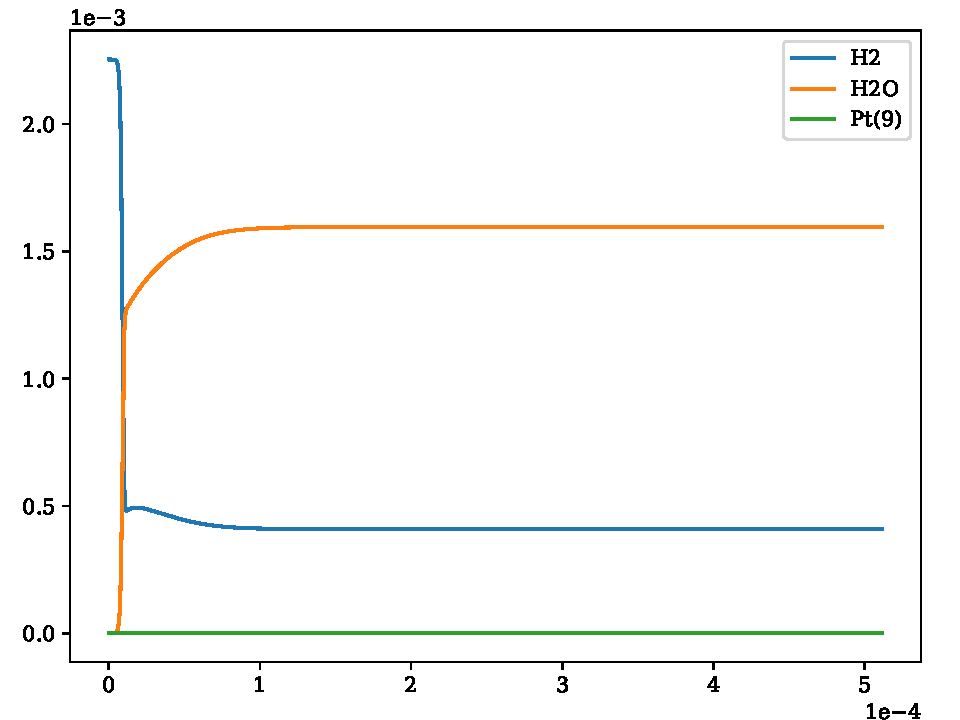
\includegraphics[scale=0.8]{figures/PlatinumLargeHydrogen_0_well_stirred_reactor.pdf}
    \caption{Selected species behavior for the well-stirred reactor over time.}
    \label{fig:wsr}
\end{figure}

Table~\ref{t1:mechanisms} lists all of the kinetics models associated with this study and some basic information about each model.
We included models of 14 different gas phase models and one surface phase model
A complete test configuration for the well stirred reactor would be a pair of a gas phase model with the surface phase model.
Including both gas and surface phases, the smallest configuration has 69 species and 740 reactions and the largest has 933 species and 7402 reactions.
Note that the combustor-exhaust problem has two reactors and consequently double the number of gas phase variables.
All of the models listed here and testing codes for the problems described are freely available on Github\cite{testing_package}.

\begin{table*}[ht] \small
    \centering
    \begin{tabular}{@{}llll@{}}
        \toprule
        Model & Formula\slash fuel name(s) & Species & Reactions\\
        \midrule
        Hydrogen~\cite{smith_gri-mech_1999} & \ce{H2} & 10 & 29\\
        GRI-Mech 3.0~\cite{smith_gri-mech_1999} & \ce{CH4} & 55 & 325\\
        Platinum~\cite{kreitz2022detailed} & \ce{Pt} & 59 & 538\\
        DME-Propane~\cite{dames_detailed_2016} & \ce{CH3OCH3} \& \ce{C3H8} & 122 & 711\\
        HyChem Jet-A~\cite{wang_physics-based_2018, xu_physics-based_2018} & POSF 10325 (\ce{C11H22}) & 203 & 1589\\
        Butane~\cite{zhang_shock_2013} & \ce{C4H10} & 230 & 2461\\
        2-Butonane~\cite{hemken_2017} & \ce{C4H8O1}-2 & 315 & 1803\\
        Isobutene~\cite{li_2016} & \textit{i-}\ce{C4H8} & 493 & 2716\\
        \textit{n}-Heptane~\cite{mehl_kinetic_2011} & \textit{n-}\ce{C7H16} & 654 & 4846\\
        Isooctane~\cite{mehl_chemical_2009} & \textit{i-}\ce{C8H18} & 874 & 6864\\
        3-Methylheptane~\cite{mehl_chemical_2009} & \ce{C8H18}\ce{-3} & 1378 & 8143\\
        \textit{n}-Hexadecane~\cite{westbrook_detailed_2007} & \textit{n-}\ce{c16h34} & 2115 & 13341\\
        Methyl-5-decenoate~\cite{herbinet_detailed_2010} & MD5D & 2649 & 10487\\
        Methyl-decanoate \& \textit{n}-heptane~\cite{herbinet_detailed_2010} & \ce{MD} \& \textit{n-}\ce{C7H16} & 3787 & 10264\\
        2-Methyl-nonadecane~\cite{sarathy_comprehensive_2011} & \ce{C20H42}-\ce{2} & 7171 & 38324\\ \hline
    \end{tabular}
    \caption{Details on the chemical kinetic models used for testing.}
    \label{t1:mechanisms}
\end{table*}

\sectionOne{Results \& discussion}

We extended generalized preconditioning to model fluid-surface chemical iteraction.
We ran the tests described in Section~\ref{sec:test-problems} to analyze performance and selected Jet-A~\cite{wang_physics-based_2018, xu_physics-based_2018} and Butane~\cite{zhang_shock_2013} for more in-depth analyses.
We selected these specific models as Jet-A
We modified these models by removing reactions associated with the assumptions made and ran the same testing configurations to understand the impact of these assumptions.
We also seek to understand the fundamental reasons behind performance impacts based on tunable parameters and assumptions made.

\sectionTwo{Performance}

In Figure~\ref{fig:nce-perf} we present the speed-up of each of the configurations.
The color of each line in the aforementioned figure describes which fuel was used and the marker indicates both the specific data points and the surface model used.
We see speed-up for the more complicated system...
\begin{figure}[htb]
    \begin{center}
        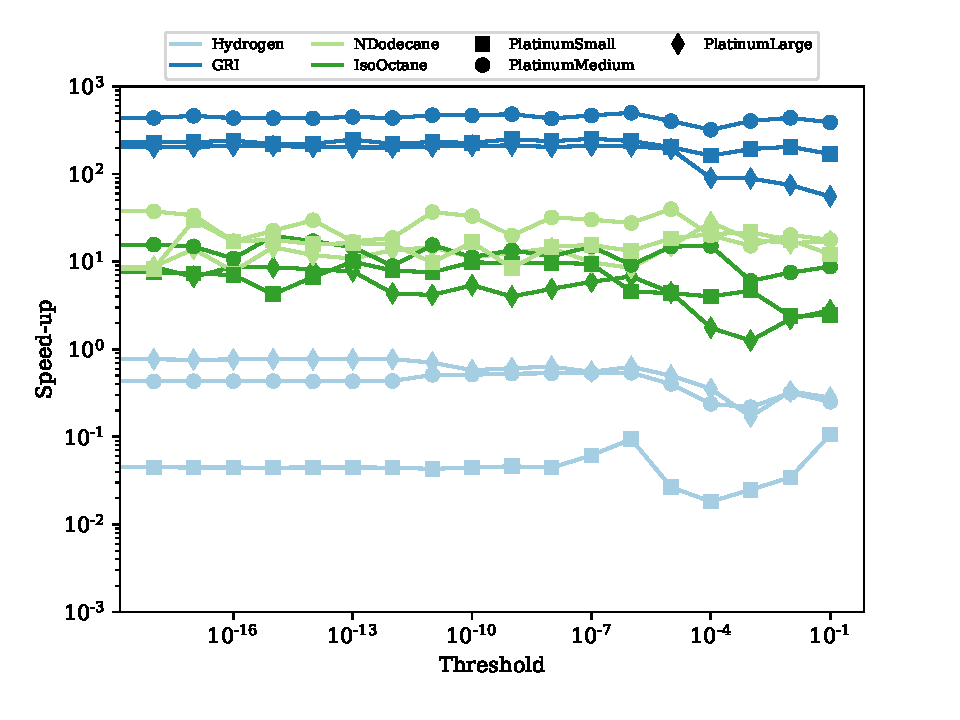
\includegraphics[width=0.9\textwidth]{figures/nce-all-models.pdf}
        \label{fig:nce-perf}
        \caption{Combustor-Exhaust system speedup for all configurations.}
    \end{center}
\end{figure}

\sectionTwo{Reaction Analysis}

We experimented with removing reactions that are associated with certain assumptions to understand the role that these assumptions play in performance.
We looked at the results from a variety of different perspectives.
We first considered the GRI gas phase model\cite{smith_gri-mech_1999} and the Small\cite{deutschmann1996numerical} and Large\cite{kreitz2022detailed} surface models.
We show the speed-up of these models in Figure~\ref{fig:gri_ra}.
Note, the legends in this figure follow the same color and marker paradigm as Figure~\ref{fig:nce-perf}.
The one caviot is that the entries may now have a suffix such as \texttt{ntb}, \texttt{nfo}, or both. These suffixes stand for "no thirdbody" and "no falloff".
These suffixes will continue to be used throughout the remaining results to differentiate the cases where these types of reactions were stripped from the models.

In Figure~\ref{fig:gri_ra}, we see that GRI with the small surface has less variation in performance cases than GRI with the large surface.
We also see a somewhat inverse behavior between the small and large surface models where the best performance for the small model is when all assumptions are removed and the best for the large surface are when no assumptions are removed.
In the small model, falloff and thirdbody reactions make up approximately 14\% of the total reactions.
In the large model, these reactions make up approximately 6\% of the total reactions.
The inverse behavior can be accounted for with this difference in composition of reactions.
When these equations are removed, the jacobian used for the preconditioner becomes closer to the exact Jacobian and consequently requires less linear iterations.
We would expect the same behavior for the large system but as the percentage of these reactions decreases the approximate and exact Jacobians become closer so the assumptions are less dominant.

\begin{figure}[htb]
    \centering
    \begin{subfigure}{0.49\textwidth}
        \centering
        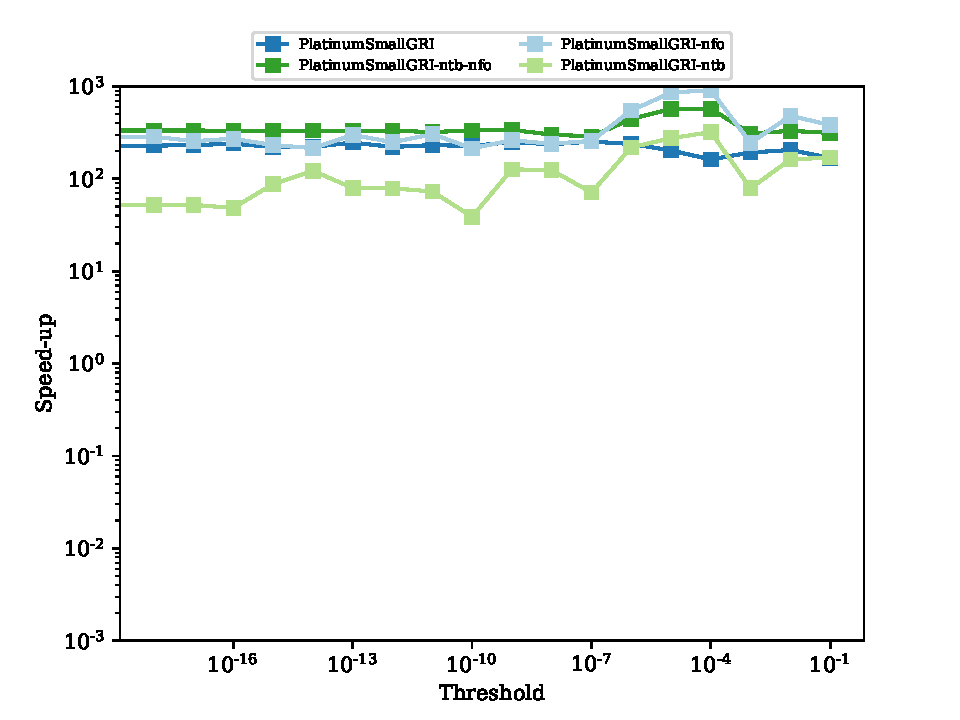
\includegraphics[width=\textwidth]{figures/speedup-gri-small-network_combustor_exhaust.pdf}
        \caption{Speed-up of PlatinumSmall and GRI cases.}
        \label{fig:gri_small_su}
    \end{subfigure}
    \hfill
    \begin{subfigure}{0.49\textwidth}
        \centering
        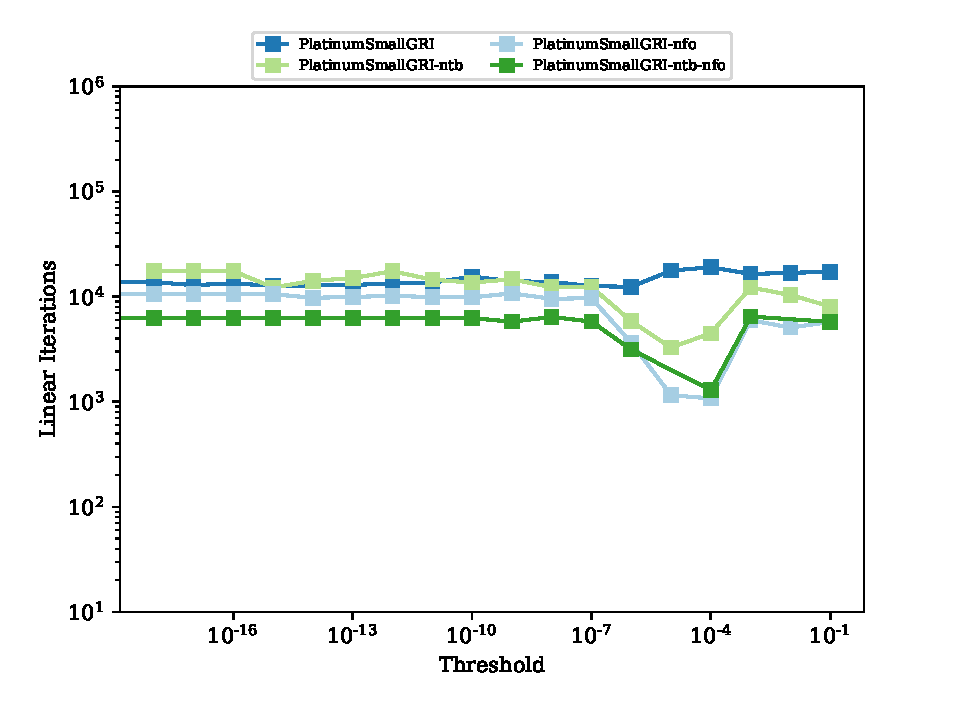
\includegraphics[width=\textwidth]{figures/lin_iters_gri_small.pdf}
        \caption{Linear iterations of PlatinumSmall and GRI cases.}
        \label{fig:gri_small_cond}
    \end{subfigure}
    \hfill

    \begin{subfigure}{0.49\textwidth}
        \centering
        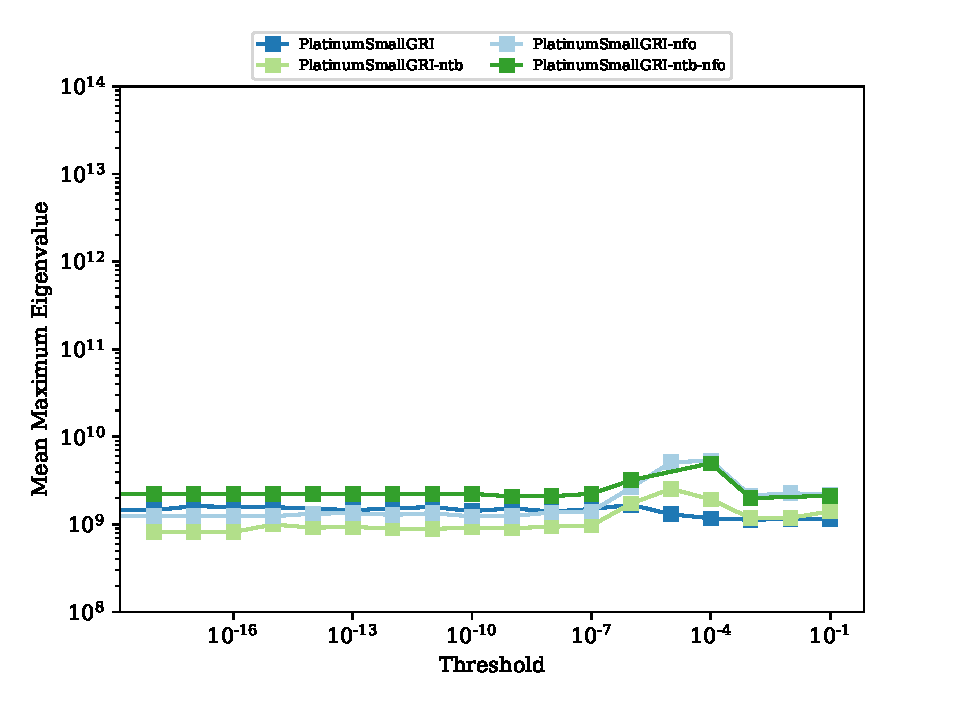
\includegraphics[width=\textwidth]{figures/max_eigen_gri_small.pdf}
        \caption{Mean maximum eigenvalue of PlatinumSmall and GRI cases.}
        \label{fig:gri_small_me}
    \end{subfigure}
    \hfill
    \begin{subfigure}{0.49\textwidth}
        \centering
        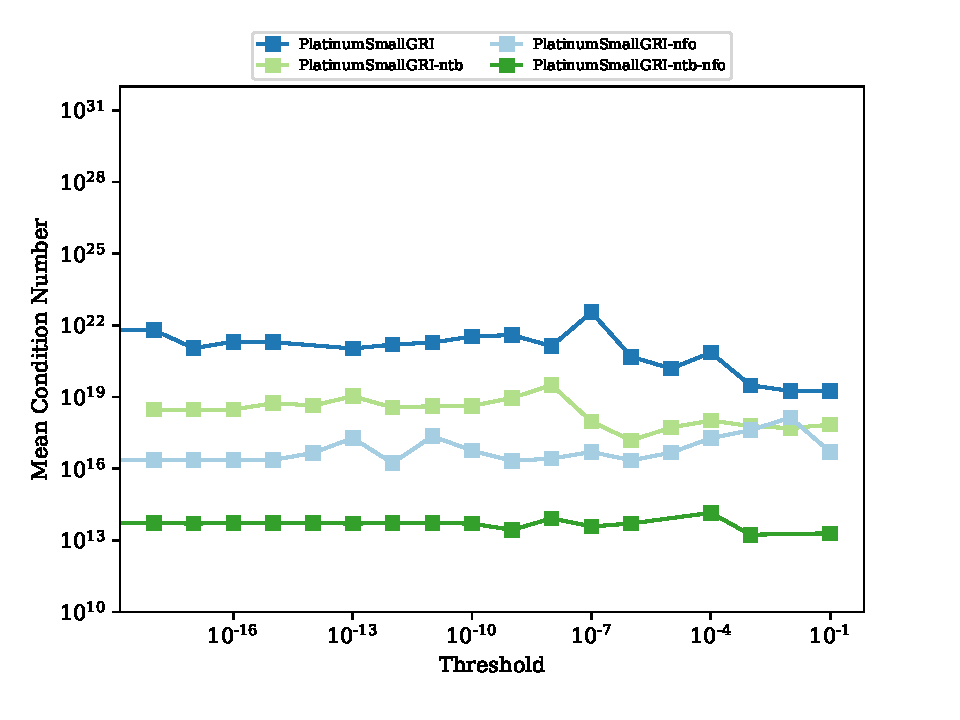
\includegraphics[width=\textwidth]{figures/condition_gri_small.pdf}
        \caption{Mean condition number of PlatinumSmall and GRI cases.}
        \label{fig:gri_small_iters}
    \end{subfigure}
    \hfill
    \caption{Analysis of PlatinumLarge with GRI in several cases.}
    \label{fig:gri_small}
\end{figure}

We want to confirm that these assumptions become less important as their percentage decreases so we consider a larger model, IsoOctane\cite{mehl_chemical_2009}, in Figure~\ref{fig:c8h18_ra}.
In this case, falloff and thirdbody reactions make up less than 1\% of both IsoOctane with the small and large surfaces.
In this figure, we see mixed behavior, where in some cases the removal of these equations improves performance and others it does not.
The mixed behavior implies that there is another factor driving the performance as the composition of thirdbody and falloff reactions decreases.

\begin{figure}[htb]
    \centering
    \begin{subfigure}{0.49\textwidth}
        \centering
        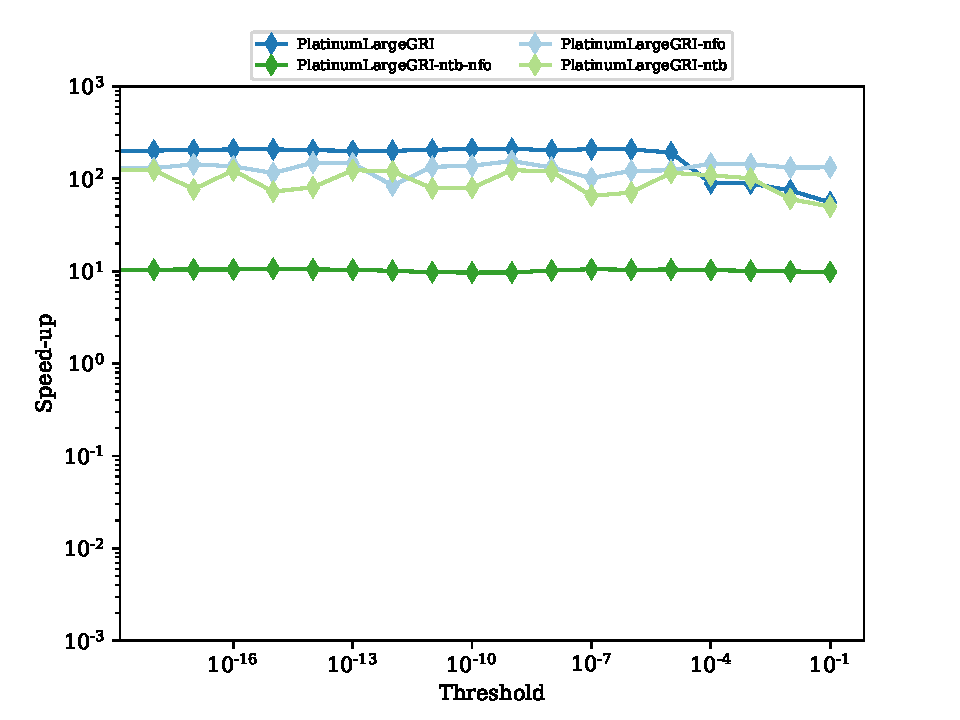
\includegraphics[width=\textwidth]{figures/speedup-gri-large-network_combustor_exhaust.pdf}
        \caption{Speed-up of PlatinumLarge and GRI cases.}
        \label{fig:gri_large_su}
    \end{subfigure}
    \hfill
    \begin{subfigure}{0.49\textwidth}
        \centering
        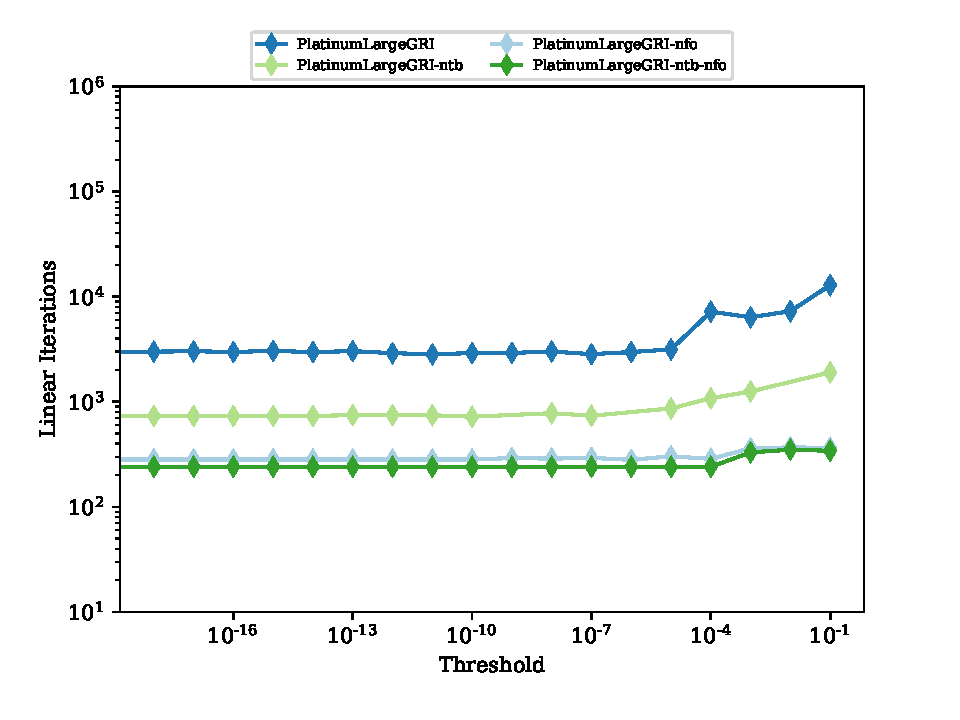
\includegraphics[width=\textwidth]{figures/lin_iters_gri_large.pdf}
        \caption{Linear iterations of PlatinumLarge and GRI cases.}
        \label{fig:gri_large_cond}
    \end{subfigure}
    \hfill

    \begin{subfigure}{0.49\textwidth}
        \centering
        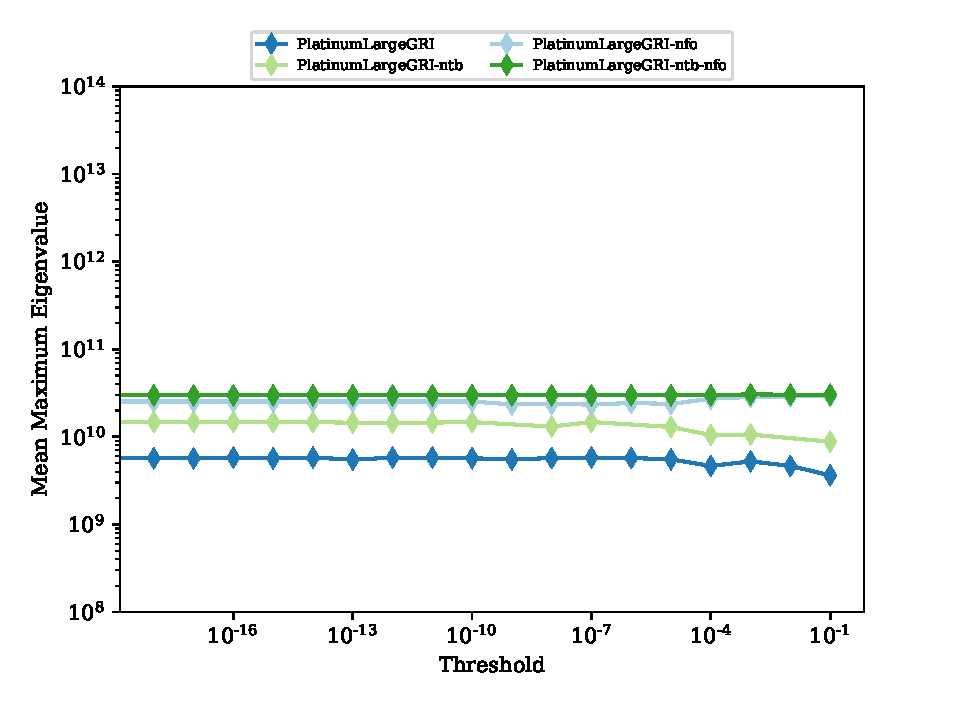
\includegraphics[width=\textwidth]{figures/max_eigen_gri_large.pdf}
        \caption{Mean maximum eigenvalue of PlatinumLarge and GRI cases.}
        \label{fig:gri_large_me}
    \end{subfigure}
    \hfill
    \begin{subfigure}{0.49\textwidth}
        \centering
        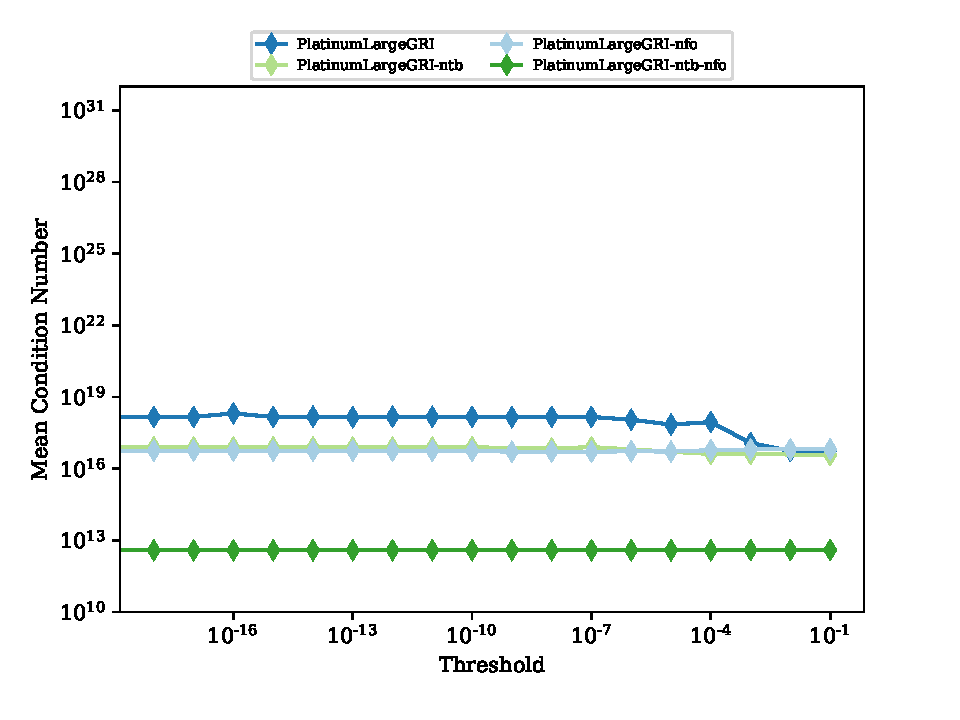
\includegraphics[width=\textwidth]{figures/condition_gri_large.pdf}
        \caption{Mean condition number of PlatinumLarge and GRI cases.}
        \label{fig:gri_large_iters}
    \end{subfigure}
    \hfill
    \caption{Analysis of PlatinumLarge with GRI in several cases.}
    \label{fig:gri_large}
\end{figure}


\begin{figure}[htb]
    \centering
    \begin{subfigure}{0.49\textwidth}
        \centering
        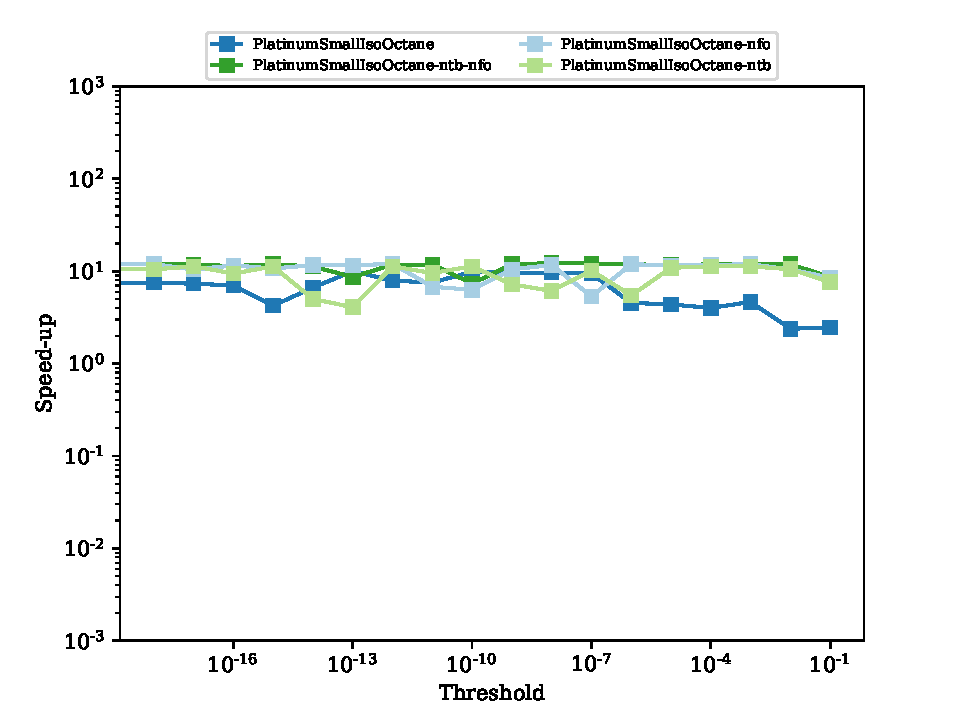
\includegraphics[width=\textwidth]{figures/speedup-isooctane-small-network_combustor_exhaust.pdf}
        \caption{Speed-up of PlatinumLarge and GRI cases.}
        \label{fig:isooctane_small_su}
    \end{subfigure}
    \hfill
    \begin{subfigure}{0.49\textwidth}
        \centering
        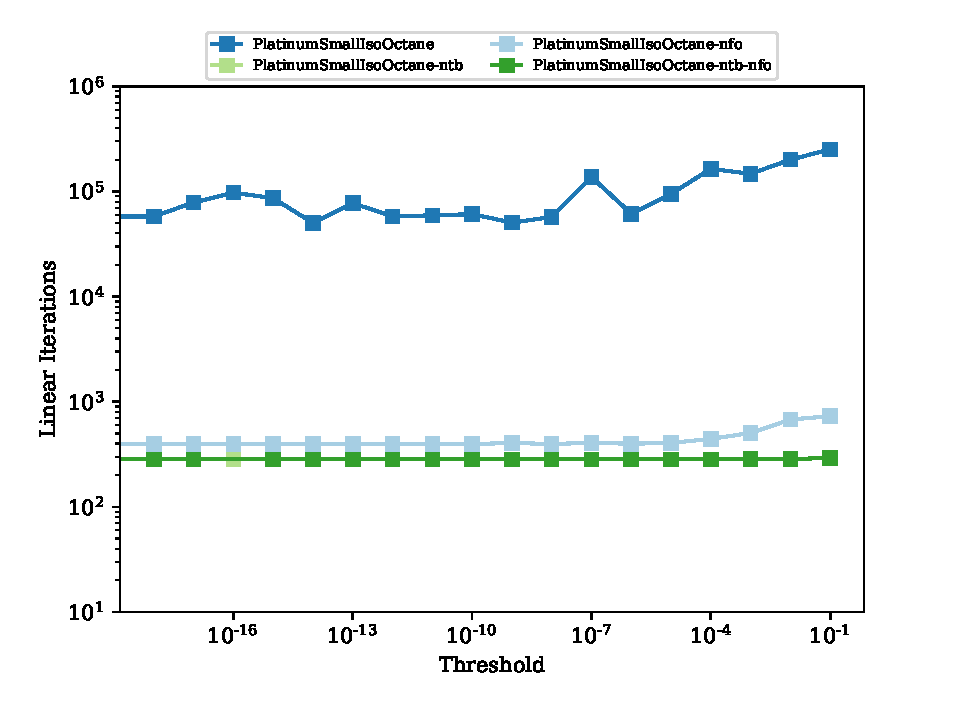
\includegraphics[width=\textwidth]{figures/lin_iters_isooctane_small.pdf}
        \caption{Linear iterations of PlatinumLarge and GRI cases.}
        \label{fig:isooctane_small_cond}
    \end{subfigure}
    \hfill

    \begin{subfigure}{0.49\textwidth}
        \centering
        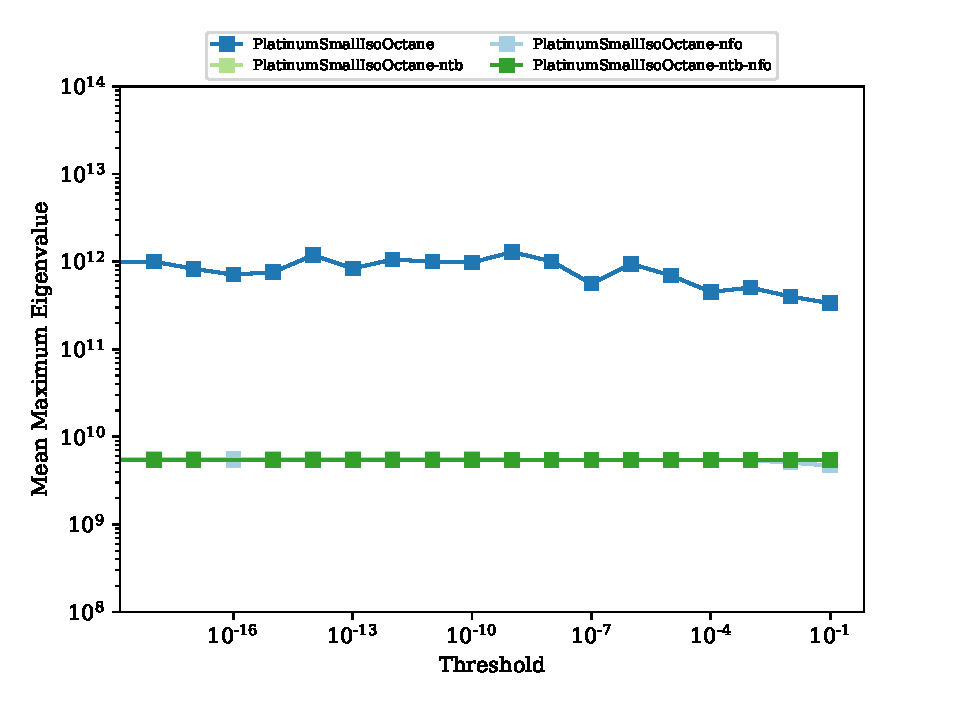
\includegraphics[width=\textwidth]{figures/max_eigen_isooctane_small.pdf}
        \caption{Mean maximum eigenvalue of PlatinumLarge and GRI cases.}
        \label{fig:isooctane_small_me}
    \end{subfigure}
    \hfill
    \begin{subfigure}{0.49\textwidth}
        \centering
        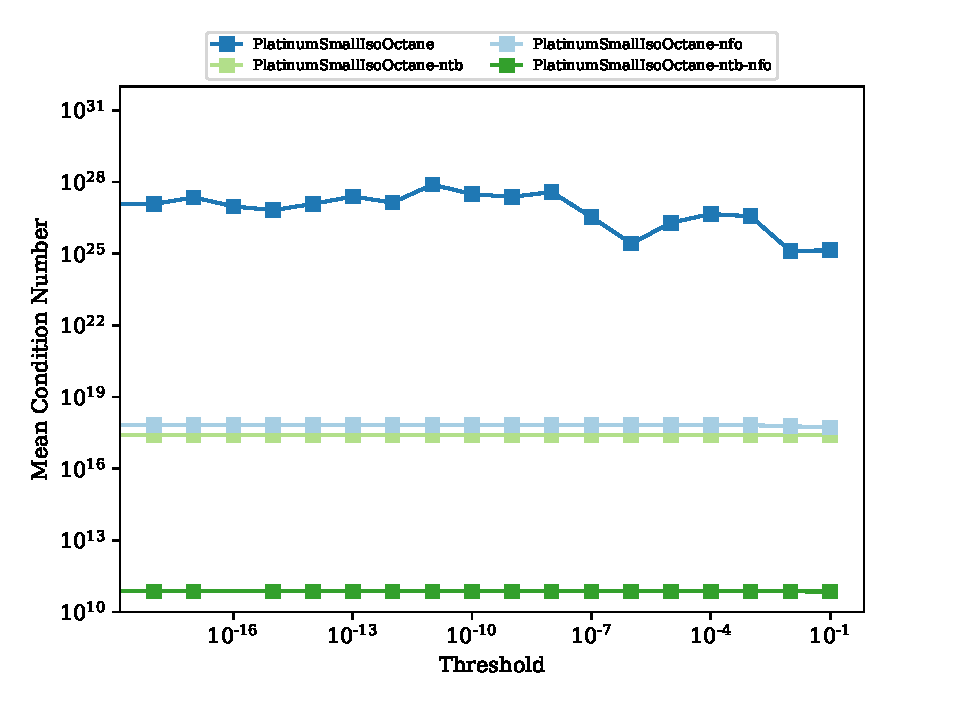
\includegraphics[width=\textwidth]{figures/condition_isooctane_small.pdf}
        \caption{Mean condition number of PlatinumLarge and GRI cases.}
        \label{fig:isooctane_small_iters}
    \end{subfigure}
    \hfill
    \caption{Analysis of PlatinumLarge with GRI in several cases.}
    \label{fig:isooctane_small}
\end{figure}

We want to understand the driving factor behind performance and consquently we consider a more thorough analysis of these assumptions based on the threshold.
The condition number is a well-known matrix quantity used to assess the sensitivity of the solution to perturbations and round-off errors\cite{trefethen1997numerical}.
A matrix with a large condition number is said to be ill-conditioned meaning that it is more sensitive which generally makes iterative methods converge more slowly.
The performance of an iterative linear method is dependent on it's ability to converge more quickly.
Consequently, we consider the mean condition number of these cases in Figure~\ref{fig:gri_cond}.


When we compare Figures~\ref{fig:gri_ra} and~\ref{fig:gri_cond}, we see that Figure~\ref{fig:gri_small_cond} matches our expectation that a large condition number leads to poorer performance but Figure~\ref{fig:gri_large_cond} does not.
We expect the condition number of the matrix to inversely correlate with performance but it becomes substantially less dominate with lower orders of magnitude.
We see that Figures~\ref{fig:gri_large_ra} and~\ref{fig:gri_large_cond} match very well qualitatively.
Stiffness is also dominating the system...


\sectionTwo{Thresholding Analysis}

\sectionOne{Conclusions}

\printbibliography

\end{document}

% -------------------------------------------------------------------- %
% -------------------------------------------------------------------- %
% -------------------------------------------------------------------- %
